\chapter{研究方法}
\fontsize{12pt}{18pt}\selectfont

% ------------------------- 3.0 ------------------------- %
% 研究目的;研究假設;研究方法
本研究目的是透過最佳化方法估計肌肉參數,省去醫療器材量測之高成本,藉以生成個人化模型,
應用於復健規劃、運動訓練與輔具設計等領域。本研究假設為已知一肌肉骨骼模型,該模型除了欲評估之肌肉參數外,
其餘幾何特徵、肌肉參數等資訊皆為已知,而其可透過 OpenSim 軟體來執行任何模擬。研究方法主要分為三大主軸,
介紹如下:
\begin{itemize}
    \item \textbf{主軸一:敏感度分析}
    \\ 透過擾動肌肉參數,來計算出任務與參數間之敏感度,其指標是藉由預測任務之誤差來表示。
       敏感度高意味著該肌肉和該任務具有高相關性,其結果提供最佳化與模型驗證之任務挑選的參考依據。
    \item \textbf{主軸二:多運動軌跡預測最佳化}
    \\ 從敏感度分析挑選數個適當任務作為輸入,並將多運動軌跡預測任務之平均預測誤差視作目標函數,
       藉由最佳化方法最小化平均預測誤差,以此估計出最佳模型之肌肉參數。   
    \item \textbf{主軸三:模型驗證}
    \\ 從敏感度分析挑選適當任務作為輸入,指定最佳模型完成並檢視其預測誤差,
       確認該模型是否於其它任務仍具有低誤差表現,以此驗證模型正確性。
\end{itemize}

% 研究流程圖 + 說明
本研究之流程圖如圖 \ref{ch3_flowchart_All} 所示,首先輸入標準模型和分析參數來執行敏感度分析,
藉由全因子實驗設計法來評估出所有任務之敏感度指標,接下來挑選適合的組合集作為最佳化之評估任務,
以生成最佳模型,最終透過高敏感度任務進行模型驗證,來評估最佳模型之正確性。
若於模型驗證階段成功,代表評估正確,並結束程式執行;若於模型驗證階段失敗,則返回至最佳化步驟重新評估;
若模型驗證失敗次數過多,則返回至敏感度分析流程,重新挑選合適的評估任務。
程式碼將發布於 https://github.com/solab-ntu/MuscleParamEstimation 該網址中,執行細節可檢視程式碼中的註解說明。

\bigskip
\begin{figure}[!ht]
	\centering
	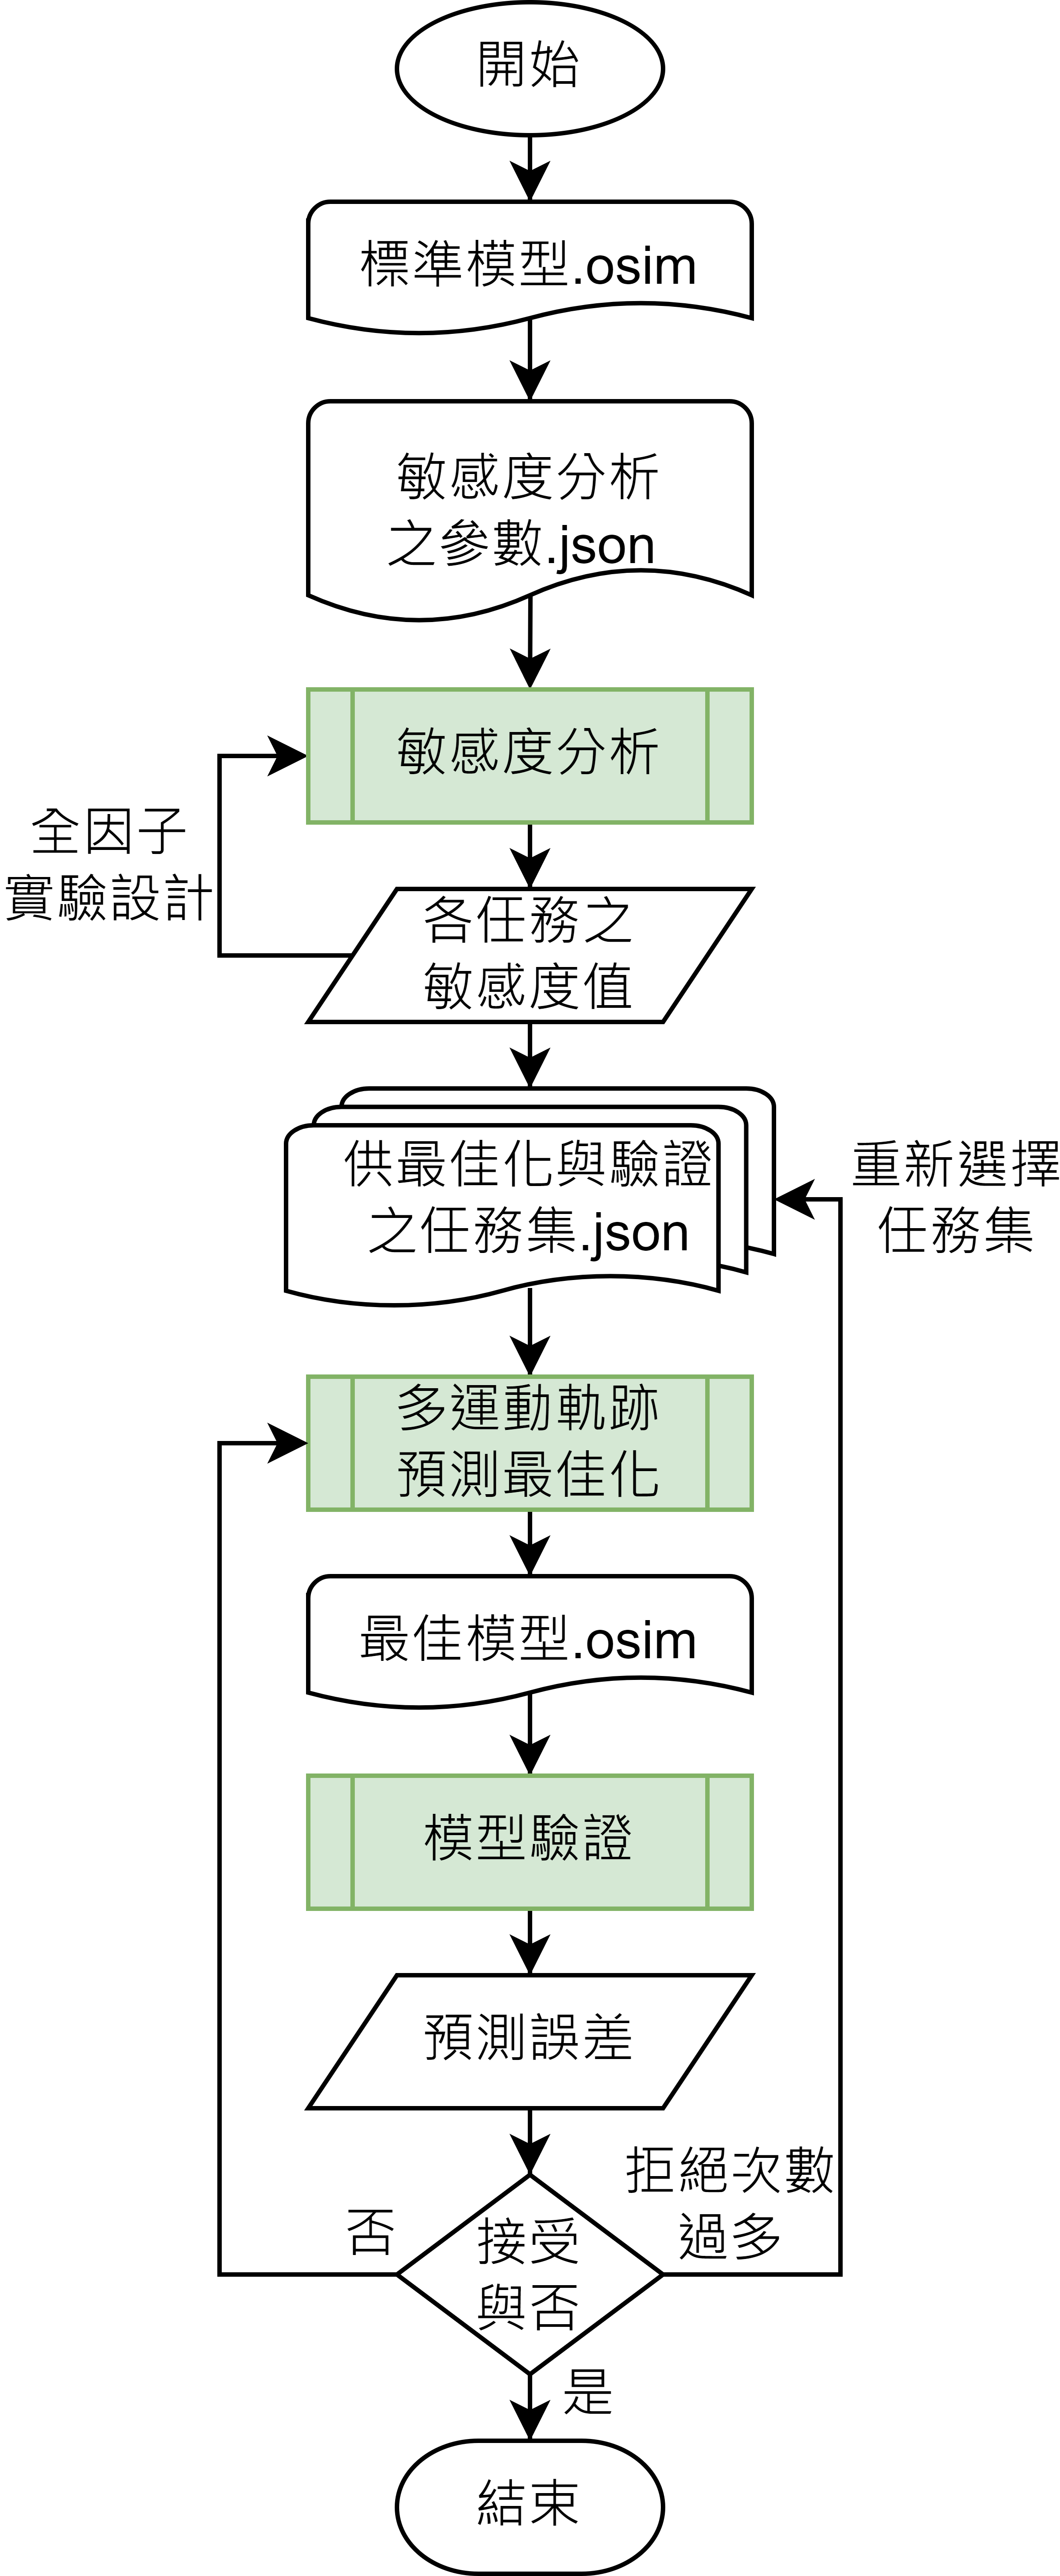
\includegraphics[width=8cm]{figure/ch3_flowchart_All.png}
    \caption[研究總流程圖]{研究總流程圖}
    \label{ch3_flowchart_All}
\end{figure}

\clearpage

% ------------------------- 3.1 ------------------------- %
\section{系統架設與實驗環境}
% 系統架設;實驗環境

\subsection{系統架設}
% 系統架設介紹
123123
\subsubsection{硬體-相機擺放}
% 硬體介紹;相機擺放
123123
\subsubsection{軟體-xsens}
% 軟體介紹;xsens
123123

\subsection{實驗環境}
% 實驗環境介紹
123123

% ------------------------- 3.2 ------------------------- %
\section{資料前處理}
% 資料前處理介紹
123123

\subsection{人體骨架建立}
% 人體骨架建立介紹
pose2sim

\subsection{時間軸對齊}
% 時間軸對齊介紹
拍手及加速度判斷

\subsection{IMU - 全域座標轉換矩陣計算}
% IMU - 全域座標轉換矩陣計算介紹
$R_{ig}$

\subsection{IMU - 骨架座標轉換矩陣計算}
% IMU - 骨架座標轉換矩陣計算介紹
$R_{ib}$

% ------------------------- 3.3 ------------------------- %
\section{探討減少相機數量的可行性及其擺放位置}
% 探討減少相機數量的可行性及其擺放位置介紹
total capture dataset 的資料總共包含 8 台相機與 13 個 IMU 的 data,
而在 Fusing wearable imus with multi-view images 中,作者表明他只使用到 4 台相機及 8 個 IMU 的資料;
另外在 total capture 發表的文獻中則有提到他們嘗試減少相機的硬體數量,準確度隨著相機數量的減少而下降,
因此本章節嘗試選擇相機數量與位置並進行感測器融合計算,
將得到的結果與 total capture dataset 提供的 Vicon 資料進行比對,計算 MPJPE,
藉此方式欲探討相機數量的減少對於動作捕捉的影響,並嘗試探討相機擺放位置的選擇。

\subsection{實驗方法-數量及位置選擇}
% 實驗方法介紹
% 目前的相機用量及擺放位置敘述,要 cite totalcapture 和 data fusion
從 total capture dataset 提供的影像資料可以觀察出其實驗環境為一個方形的空間,每一面牆面上方架設兩台相機,
四面牆共計八台相機,擺放位置如圖 所示。
\subsubsection{四台相機}
將圖 中的相機進行排列組合,共計有 70 種組合方式,每一種組合方式皆會產生一組 MPJPE,
結果如表 \ref{ch3_cameraset_4cam}所示,其中最佳組合方式為相機 1357,其 MPJPE 為 24.5789(mm);
而最差組合方式為相機 2567,其 MPJPE 為 38.9142(mm)。標準差為 3.6860(mm),平均值為 31.0114(mm)。
經由標準差可以知道四台相機組合的表現都相當穩定,無論如何選擇都不會有太大的影響。
\begin{table}[!ht]
   \caption[四台相機組合與其估計結果誤差]{四台相機組合與其估計結果誤差}
   \centering
   \label{ch3_cameraset_4cam}
   \setlength{\tabcolsep}{3pt}
   \renewcommand\arraystretch{1.5}
   \resizebox{\textwidth}{!}{
   \begin{tabular}{|
   >{\columncolor[HTML]{E7E6E6}}c |c|
   >{\columncolor[HTML]{E7E6E6}}c |c|
   >{\columncolor[HTML]{E7E6E6}}c |c|
   >{\columncolor[HTML]{E7E6E6}}c |c|
   >{\columncolor[HTML]{E7E6E6}}c |c|}
      \midrule
      相機配置 & MPJPE & 相機配置 & MPJPE & 相機配置 & MPJPE & 相機配置 & MPJPE & 相機配置 & MPJPE \\
      \midrule
      1234 & 30.9409 & 1235 & 28.8549 & 1236 & 30.3748 & 1237 & 28.8213 & 1238 & 31.1560 \\
      1245 & 33.1706 & 1246 & 31.5377 & 1247 & 32.1031 & 1248 & 33.6613 &            &         \\
      1256 & 34.5089 & 1257 & 34.6787 & 1258 & 35.2625 &            &         &            &         \\
      1267 & 31.7009 & 1268 & 33.0636 & 1278 & 34.6861 &            &         &            &         \\
      \midrule
      1345 & 26.9753 & 1346 & 28.2925 & 1347 & 25.4715 & 1348 & 26.7584 &            &         \\
      1356 & 27.7651 & 1357 & 24.5789 & 1358 & 25.8578 &            &         &            &         \\
      1367 & 26.3845 & 1368 & 26.9445 & 1378 & 26.1466 &            &         &            &         \\
      \midrule
      1456 & 29.9311 & 1457 & 26.6848 & 1458 & 27.9429 &            &         &            &         \\
      1467 & 26.8121 & 1468 & 27.5472 & 1478 & 27.1979 &            &         &            &         \\
      \midrule
      1567 & 27.5824 & 1568 & 29.1892 & 1578 & 27.4552 & 1678 & 27.8378 &            &         \\
      \midrule
      2345 & 34.0972 & 2346 & 36.5508 & 2347 & 36.7314 & 2348 & 33.7047 &            &         \\
      2356 & 35.6585 & 2357 & 36.3698 & 2358 & 30.8585 &            &         &            &         \\
      2367 & 36.8662 & 2368 & 32.6160 & 2378 & 34.8430 &            &         &            &         \\
      \midrule
      2456 & 35.6440 & 2457 & 37.1359 & 2458 & 33.4067 &            &         &            &         \\
      2467 & 35.8266 & 2468 & 33.2654 & 2478 & 36.6081 &            &         &            &         \\
      2567 & 38.9142 & 2568 & 33.7187 & 2578 & 38.7211 & 2678 & 34.3506 &            &         \\
      \midrule
      3456 & 32.4429 & 3457 & 27.7338 & 3458 & 27.6554 &            &         &            &         \\
      3467 & 31.0735 & 3468 & 29.9925 & 3478 & 27.9168 &            &         &            &         \\
      3567 & 29.2876 & 3568 & 28.3170 & 3578 & 26.8460 & 3678 & 29.4004 &            &         \\
      \midrule
      4567 & 29.8717 & 4568 & 29.7963 & 4578 & 28.2055 & 4678 & 28.9104 & 5678 & 29.5824 \\
      \midrule
   \end{tabular}}
\end{table}

\subsubsection{三台相機}
\begin{table}[!ht]
   \caption[三台相機組合與其估計結果誤差]{三台相機組合與其估計結果誤差}
   \centering
   \label{ch3_cameraset_3cam}
   \setlength{\tabcolsep}{3pt}
   \renewcommand\arraystretch{1.5}
   \resizebox{\textwidth}{!}{
   \begin{tabular}{|
   >{\columncolor[HTML]{E7E6E6}}c |c|
   >{\columncolor[HTML]{E7E6E6}}c |c|
   >{\columncolor[HTML]{E7E6E6}}c |c|
   >{\columncolor[HTML]{E7E6E6}}c |c|
   >{\columncolor[HTML]{E7E6E6}}c |c|}
      \midrule
      相機配置 & MPJPE & 相機配置 & MPJPE & 相機配置 & MPJPE & 相機配置 & MPJPE \\
      \midrule
      123 & 41.8538 & 124 & 43.2544 & 125 & 70.4747 & 126 & 41.7470 \\
      127 & 54.5721 & 128 & 46.7714 & & & & \\
      \midrule
      134 & 30.9862 & 135 & 29.0275 & 136 & 33.6116 & 137 & 27.1579 \\
      138 & 29.9961 & & & & & & \\
      \midrule
      145 & 34.4860 & 146 & 32.7227 & 147 & 29.9785 & 148 & 31.5573 \\
      \midrule
      156 & 38.3802 & 157 & 33.2107 & 158 & 33.4297 & & \\
      \midrule
      167 & 32.4098 & 168 & 33.4044 & 178 & 32.2636 & & \\
      \midrule
      234 & 52.0193 & 235 & 76.4435 & 236 & 52.6657 & 237 & 65.5297 \\
      238 & 44.5936 & & & & & & \\
      \midrule
      245 & 76.6047 & 246 & 42.4841 & 247 & 54.8719 & 248 & 45.2496 \\
      \midrule
      256 & 74.8608 & 257 & 82.8158 & 258 & 62.4336 & & \\
      \midrule
      267 & 58.7578 & 268 & 39.2619 & 278 & 62.7102 & & \\
      \midrule
      345 & 35.9928 & 346 & 42.7418 & 347 & 35.2381 & 348 & 33.5695 \\
      \midrule
      356 & 42.9933 & 357 & 35.1894 & 358 & 29.6995 & & \\
      \midrule
      367 & 40.0411 & 368 & 35.8360 & 378 & 34.9221 & & \\
      \midrule
      456 & 40.0658 & 457 & 37.2030 & 458 & 32.7289 & & \\
      \midrule
      467 & 35.6906 & 468 & 33.8860 & 478 & 35.3151 & & \\
      \midrule
      567 & 41.5287 & 568 & 34.8289 & 578 & 37.5083 & & \\
      \midrule
      678 & 34.8273 & & & & & & \\
      \midrule
   \end{tabular}}
\end{table}

\subsubsection{兩台相機}
\begin{table}[!ht]
   \caption[兩台相機組合與其估計結果誤差]{兩台相機組合與其估計結果誤差}
   \centering
   \label{ch3_cameraset_2cam}
   \setlength{\tabcolsep}{3pt}
   \renewcommand\arraystretch{1.5}
   \resizebox{\textwidth}{!}{
   \begin{tabular}{|
   >{\columncolor[HTML]{E7E6E6}}c |c|
   >{\columncolor[HTML]{E7E6E6}}c |c|
   >{\columncolor[HTML]{E7E6E6}}c |c|
   >{\columncolor[HTML]{E7E6E6}}c |c|
   >{\columncolor[HTML]{E7E6E6}}c |c|}
      \midrule
      相機配置 & MPJPE & 相機配置 & MPJPE & 相機配置 & MPJPE & 相機配置 & MPJPE \\
      \midrule
      12 & 194.4957 & 13 & 81.9440 & 14 & 47.4927 & 15 & 76.7795 \\
      16 & 66.8653 & 17 & 58.7619 & 18 & 46.9798 & & \\
      \midrule
      23 & 227.5722 & 24 & 182.6378 & 25 & 300.1637 & 26 & 183.0773 \\
      27 & 181.6520 & 28 & 145.2458 & & & &\\
      \midrule
      34 & 99.3426 & 35 & 109.4178 & 36 & 92.7550 & 37 & 97.7435 \\
      38 & 81.3640 & & & & & &\\
      \midrule
      45 & 87.4750 & 46 & 66.8800 & 47 & 67.4949 & 48 & 52.3318 \\
      \midrule
      56 & 126.3387 & 57 & 95.1469 & 58 & 64.6374 & &\\
      \midrule
      67 & 100.7632 & 68 & 63.7904 & & & &\\
      \midrule
      78 & 77.1948 & & & & & &\\
      \midrule
   \end{tabular}}
\end{table}

\subsection{結果}
% 結果介紹
123123
\subsection{結論}
% 結論介紹
123123

% ------------------------- 3.4 ------------------------- %
\section{結果可視化}
% 結果可視化介紹
還沒想到要寫甚麼

% ------------------------- 3.5 ------------------------- %
\section{小結}
% 本章架構
本章節首先介紹將會使用到的背景知識,像是透過希爾式肌肉模型來模擬肌肉,藉此理解肌肉的機械與生理特性,
而藉由 OpenSim 的協助,不但能快速建立肌肉骨骼模型,還可以執行正向動力學與肌肉計算控制等模擬,
且得到一個可信的結果,接下來介紹本研究的核心模擬——運動軌跡預測任務,後續的敏感度分析、最佳化過程與模型驗證,
皆是以預測任務為基礎來延伸,透過預測任務來檢視模型的表現,亦即預測誤差。
本研究透過敏感度分析來得知肌肉與任務之間的關係,藉此挑選合適的任務集作為參數評估輸入,
搭配最佳化演算法來進行參數估計,其中多組預測任務具有讓目標函數更加明確的功用,避免參數不具識別性的原因,
掉入至局部最小值結果當中,最終透過間接方法來驗證模型的正確性。

% 應用
該研究方法之應用可分為兩種討輪,第一是模擬研究,即為本研究使用之方法,透過純模擬研究來檢視該方法的可行性,
優點是其具有明確答案可供參考,且無需考慮量測造成的不確定性,在進入到實際應用前,也必須先確認模擬研究是可執行的;
第二種則是實際應用,其可透過 EMG 與動作捕捉系統來達成,藉由 EMG 量測肌肉訊號作為輸入,
動作捕捉系統量測運動軌跡作為輸出之結果比較,兩者結合並搭配本研究之最佳化方法,即可達成肌肉之參數估計,
但存在龐大的量測不確定性情況下,由於微小的軌跡偏離,即會造成肌肉參數的變動與抗衡,
縱使估計出肌肉參數,其結果之正確性仍有待商榷,因此於現今之科技發展,要達成實際應用仍有一段距離。

% 下一章節
本章節主要介紹論文之研究方法,下章節會以實際模型與動作進行討論,藉由上方所提及之方法與流程,
針對模型進行肌肉參數評估的前置作業與套用說明。

\clearpage